\section{The CERN Accelerator Complex}

CERN (Organisation europeene pour la recherche nucleaire) is a particle physics laboratory near Geneva, Switzerland crossing the Franco-Swiss border between the Swiss commune of Meyrin and French town of Saint-Genis Pouilly. It was founded in 1952 with the creation of the Coseil Europ\'{e}en pour la Recherche Nucl\'{e}aire, which became the Organisation in 1954. It houses an accelerator complex (shown in Fig.~\ref{fig:CERN-acc-complex}) ranging in energies from hundreds of MeV (extraction energy for Linac2) to energies of 7TeV (for the LHC), delivering proton bunches to various experiments (fixed target, colliding and beam) at all energy levels. These experiments have a variety of aims, varying from neutrino physics[cite CNGS], neutron physics[cite nTOF] antimatter experiments [cite ALPHA, ASACUSA, ATRAP] as well as radio isotope [cite ISOLDE] and hadron therapy [cite ACE] research. The Large Hadron Collider (LHC), the largest accelerator at CERN, is at the forefront of high-energy physics designed to push the energy frontier of knowledge of particle physics.

\begin{figure}
\begin{center}
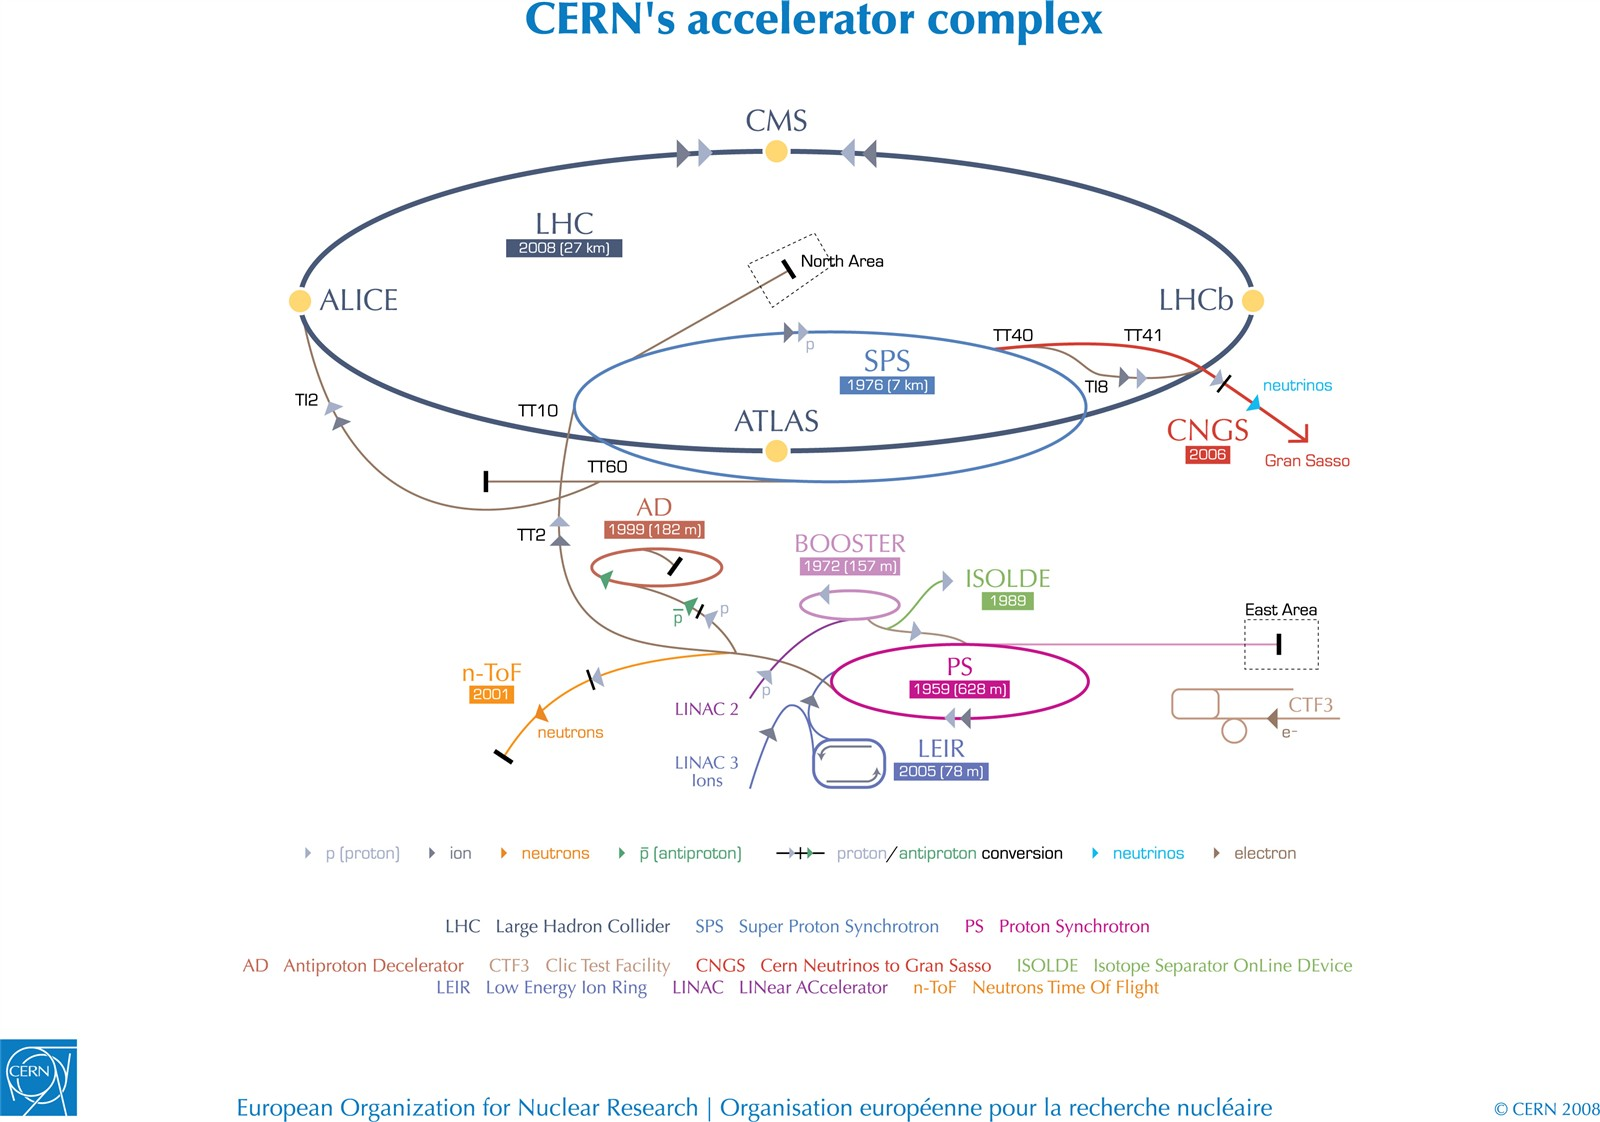
\includegraphics[width=0.95\textwidth]{Introduction/figures/cernaccelerators.jpg}
\end{center}
\label{fig:CERN-acc-complex}
\caption{The CERN accelerator complex, showing both the proton and heavy ion (lead) accelerator chains from LINACs 2 and 3 up to the LHC. Different experimental uses are highlighted in the diagram.}
\end{figure}

\section{The LHC}

The LHC is a proton synchrotron built to collide counter rotating beams of protons at an centre of mass energy of 14TeV. It uses 1,232 superconducting dipole magnets to bend the proton beams on a circular orbit around the beam line, in addition to using 392 quadrupole magnets for focusing in the transverse plane to maintain the bunch cross section and carry out final focusing for the 4 detector experiments in the LHC. Four detector experments are operated at the LHC; two general purpose detectors ATLAS and CMS, used for searches of new physics beyond the current energy frontier [cite design reports]; LHCb, a forward detector specialised in the analysis of B-physics [cite report] and ALICE, a detector specialised in heavy ion collisions with the intent of observing the physics of quark-gluon plasma [cite report. Technical Proposals]. Three further experiments are in place in the LHC, LHCf (an experiment related to the effects of high-energy cosmic rays), TOTEM (measuring the total cross-section of the proton via elastic scattering processes at the collision points) and MoEDAL (an experiment searching for magnetic monopoles and stable massive particles) complete the experiments provided with data by collisions using LHC delivered protons.

\section{Operational Figure of Merit - Luminosity}

One of the key figures of merit for the operation of the LHC (along with the centre of mass energy) is the luminosity at the colliding interaction regions (IRs). This is a figure which denotes the total rate of production of new (in the sense of produced during interactions during collisions between protons) particles in collider experiments. It can be thought of as the factor proportionality between the cross section of a reaction scheme and the number of interactions per second

\begin{equation} 
\frac{dR}{dt} = \mathcal{L} \times \sigma_{p}
\end{equation}

where $\frac{dR}{dt}$ is the interaction rate, $\mathcal{L}$ is the luminosity and $\sigma_{p}$ is the production cross section for a given particle production scheme. For two colliding bunches, each with a gaussian transverse cross-section the luminosity can be given in a simplified form by

\begin{equation}
\mathcal{L} = \frac{N_{1} N_{2} f n_{b}}{4 \pi \sigma_{x} \sigma_{y}}
\end{equation}

where $N_{1/2}$ is the bunch population of beams 1 and 2 respectively, $f$ is the revolution frequency, $n_{b}$ is the number of colliding bunches in the machine and $\sigma_{x/y}$ are the gaussian bunch sigma in the horizontal and vertical planes respectively. Both the the bunch populations $N_{1/2}$, the revoution frequency $f$ and the number of bunches $n_{b}$ also contribute towards the DC beam current in the machine $I_{b} = N_{1} f e n_{b}$ where $e$ is the elementary electron charge. As will be seen in Sec.~\ref{sec:beam_induced_heating} the expected power loss due to beam-equipment interactions by the process of power loss is proportional to the $I_{b}^{2}$, thus it can be seen that increasing the luminosity will increase the power loss experienced by in equipment in a linear to quadratic fashion.

\subsection{Integrated Luminosity}

Following from the luminosity, the determinant of the quantity of experimental data is the integrated luminosity of an experiment $\mathcal{L}_{int}$ given by

\begin{equation}
\mathcal{L}_{int} = \int^{T}_{0} \mathcal{L} \left( t \right) dt
\end{equation}

where $T$ is the integrated collision time and $\mathcal{L} (t)$ is the time varying luminosity (typically decaying exponentially over the lifetime of any given fill of the collider[cite]), varying due to changing beam conditions and bunch populaton depletion due to collisions and particle losses. The integrated luminosity is significant as the number of a given particle production schema observed by the experiments $n_{event}$ is given by

\begin{equation}
n_{event} = \mathcal{L}_{int} \times \sigma_{p}.
\end{equation}

It can thus be seen that in addition to increasing the luminosity, maximising the available time for collisions is important to maximising data collection. This requires a high level of availability of the machine, minimising failures of key systems and the down time experienced by the machine. In particular, unavoidable waiting periods between fills are to be avoided at all costs. As is seen in Chapter~\ref{chap:mki}, long cool down times (on the order of hours, similar in magnitude to the length of the average LHC fill) for equipment that requires a specific temperature range to operate correctly are thus unacceptable during ideal operation and should be reduced to a minimum. These and other sources of reduction of the running time and luminosity (due to both beam coupling impedance and other sources of instabilities and interlock trips due to hardware mishaps) must thus be carefully studied and controlled by the technical and operations teams.

\section{Beam Dynamics}
\begin{enumerate}
\item{Introduction to CERN}
\item{Introduction to the LHC}
\item{Luminousity - The Operational Figure of Merit}
\begin{itemize}
\item{Peak Luminousity - Equation and factors that control it}
\item{Integrated Luminousity - Up time and availability is important}
\end{itemize}
\item{Beam Dynamics}
\begin{itemize}
\item{Optics and Transverse Beam Dynamics}
\item{Longitudinal Dynamics - Energy change in a cavity}
\item{Chromaticity and Dispersion}
\end{itemize}
\end{enumerate}